\chapter{Ergänzungen}
% Versicherung bei Diplomarbeiten...

\section{Evaluation}

\subsection{Screenshots aus den technischen Szenarien}
\label{Anhang:screenTechnisch}

\subsection{Screenshots aus den inhaltsbasieren Szenarien}
\label{Anhang:screenInhalt}

\subsection{Evaluationsprotokoll}
\label{Anhang:protokoll}
\begin{figure}[tbh]
    \centering
    \includegraphics[scale=0.75]{images/Evaluationsprotokoll_Zeichenfläche 1-01.png}
    \caption{Evaluationsprotokoll Seite 1}
    \label{fig:protokoll1}
\end{figure}

\begin{figure}[tbh]
    \centering
    \includegraphics[scale=0.75]{images/Evaluationsprotokoll_Zeichenfläche 1-02.png}
    \caption{Evaluationsprotokoll Seite 2}
    \label{fig:protokoll2}
\end{figure}

\subsection{Ergebnisse}
\label{Anhang:Ergebnisse}

\begin{figure}[tbh]
    \centering
    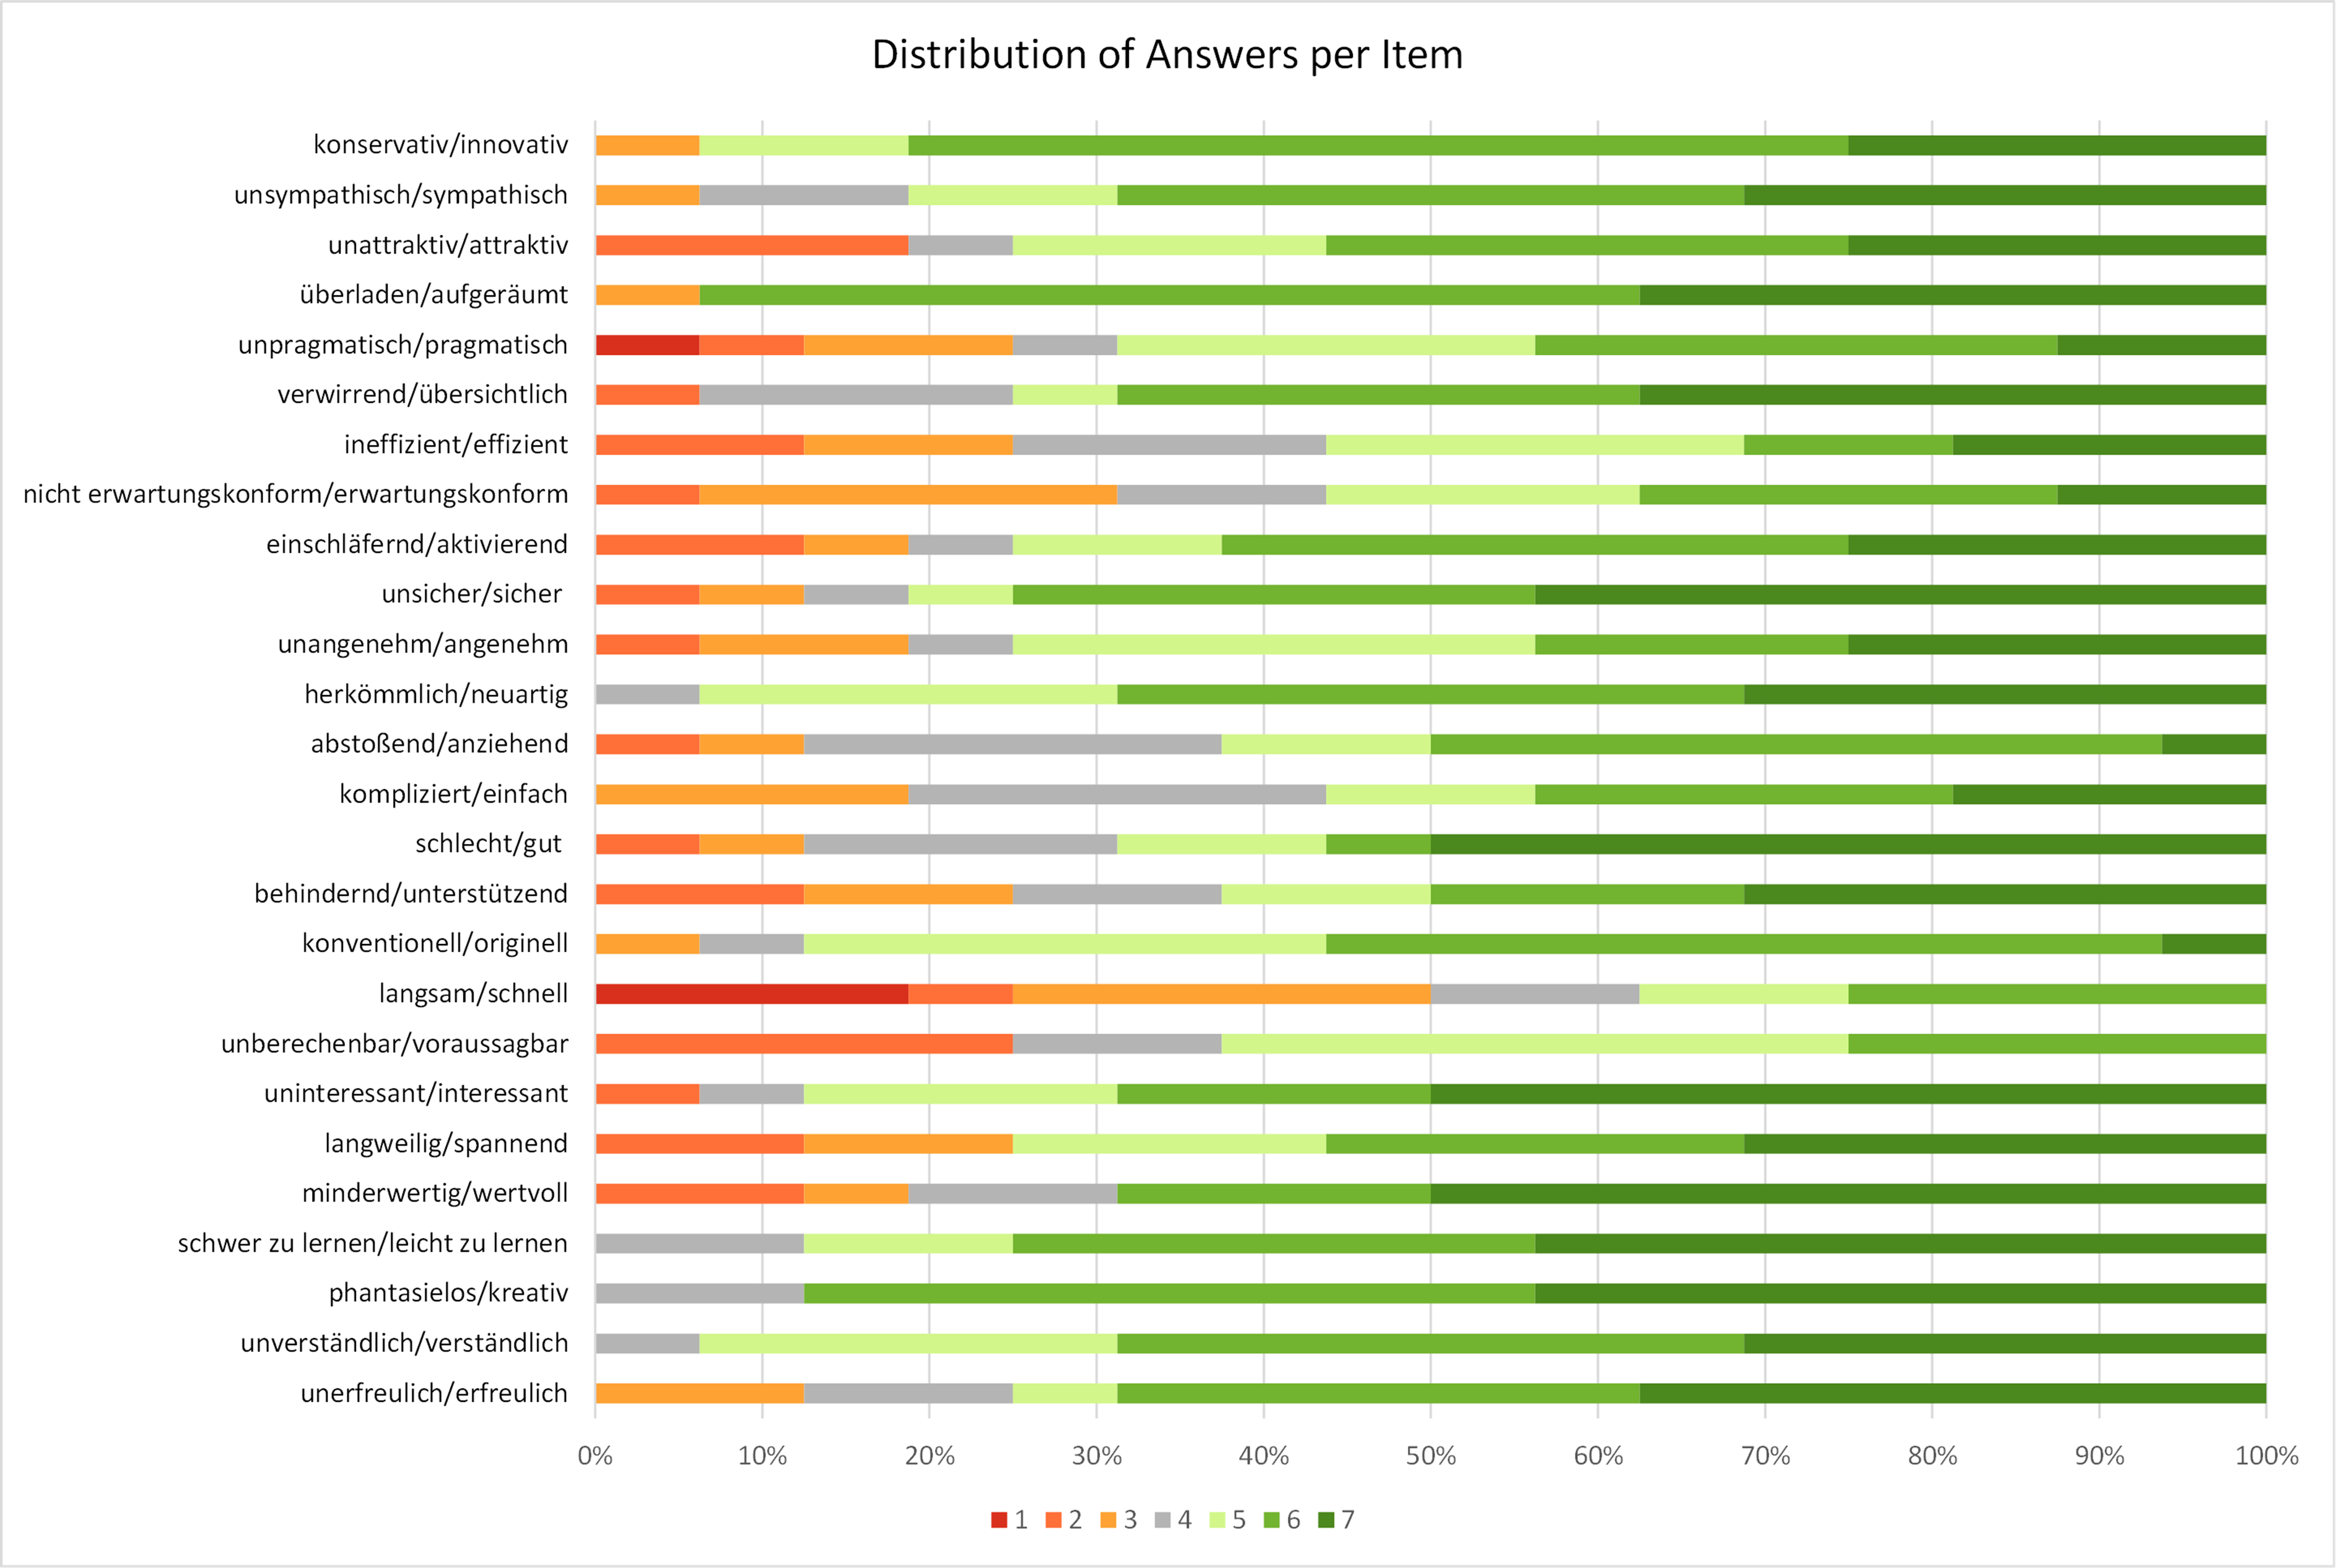
\includegraphics[scale=0.75]{images/Results/UEQ-VerteilungDerItems-ItemScanning.png}
    \caption{Genaue Verteilung der Bewertungen der Items des UEQ beim Item Scanning}
    \label{fig:ueqItemVerteilungItem}
\end{figure}

\begin{figure}[tbh]
    \centering
    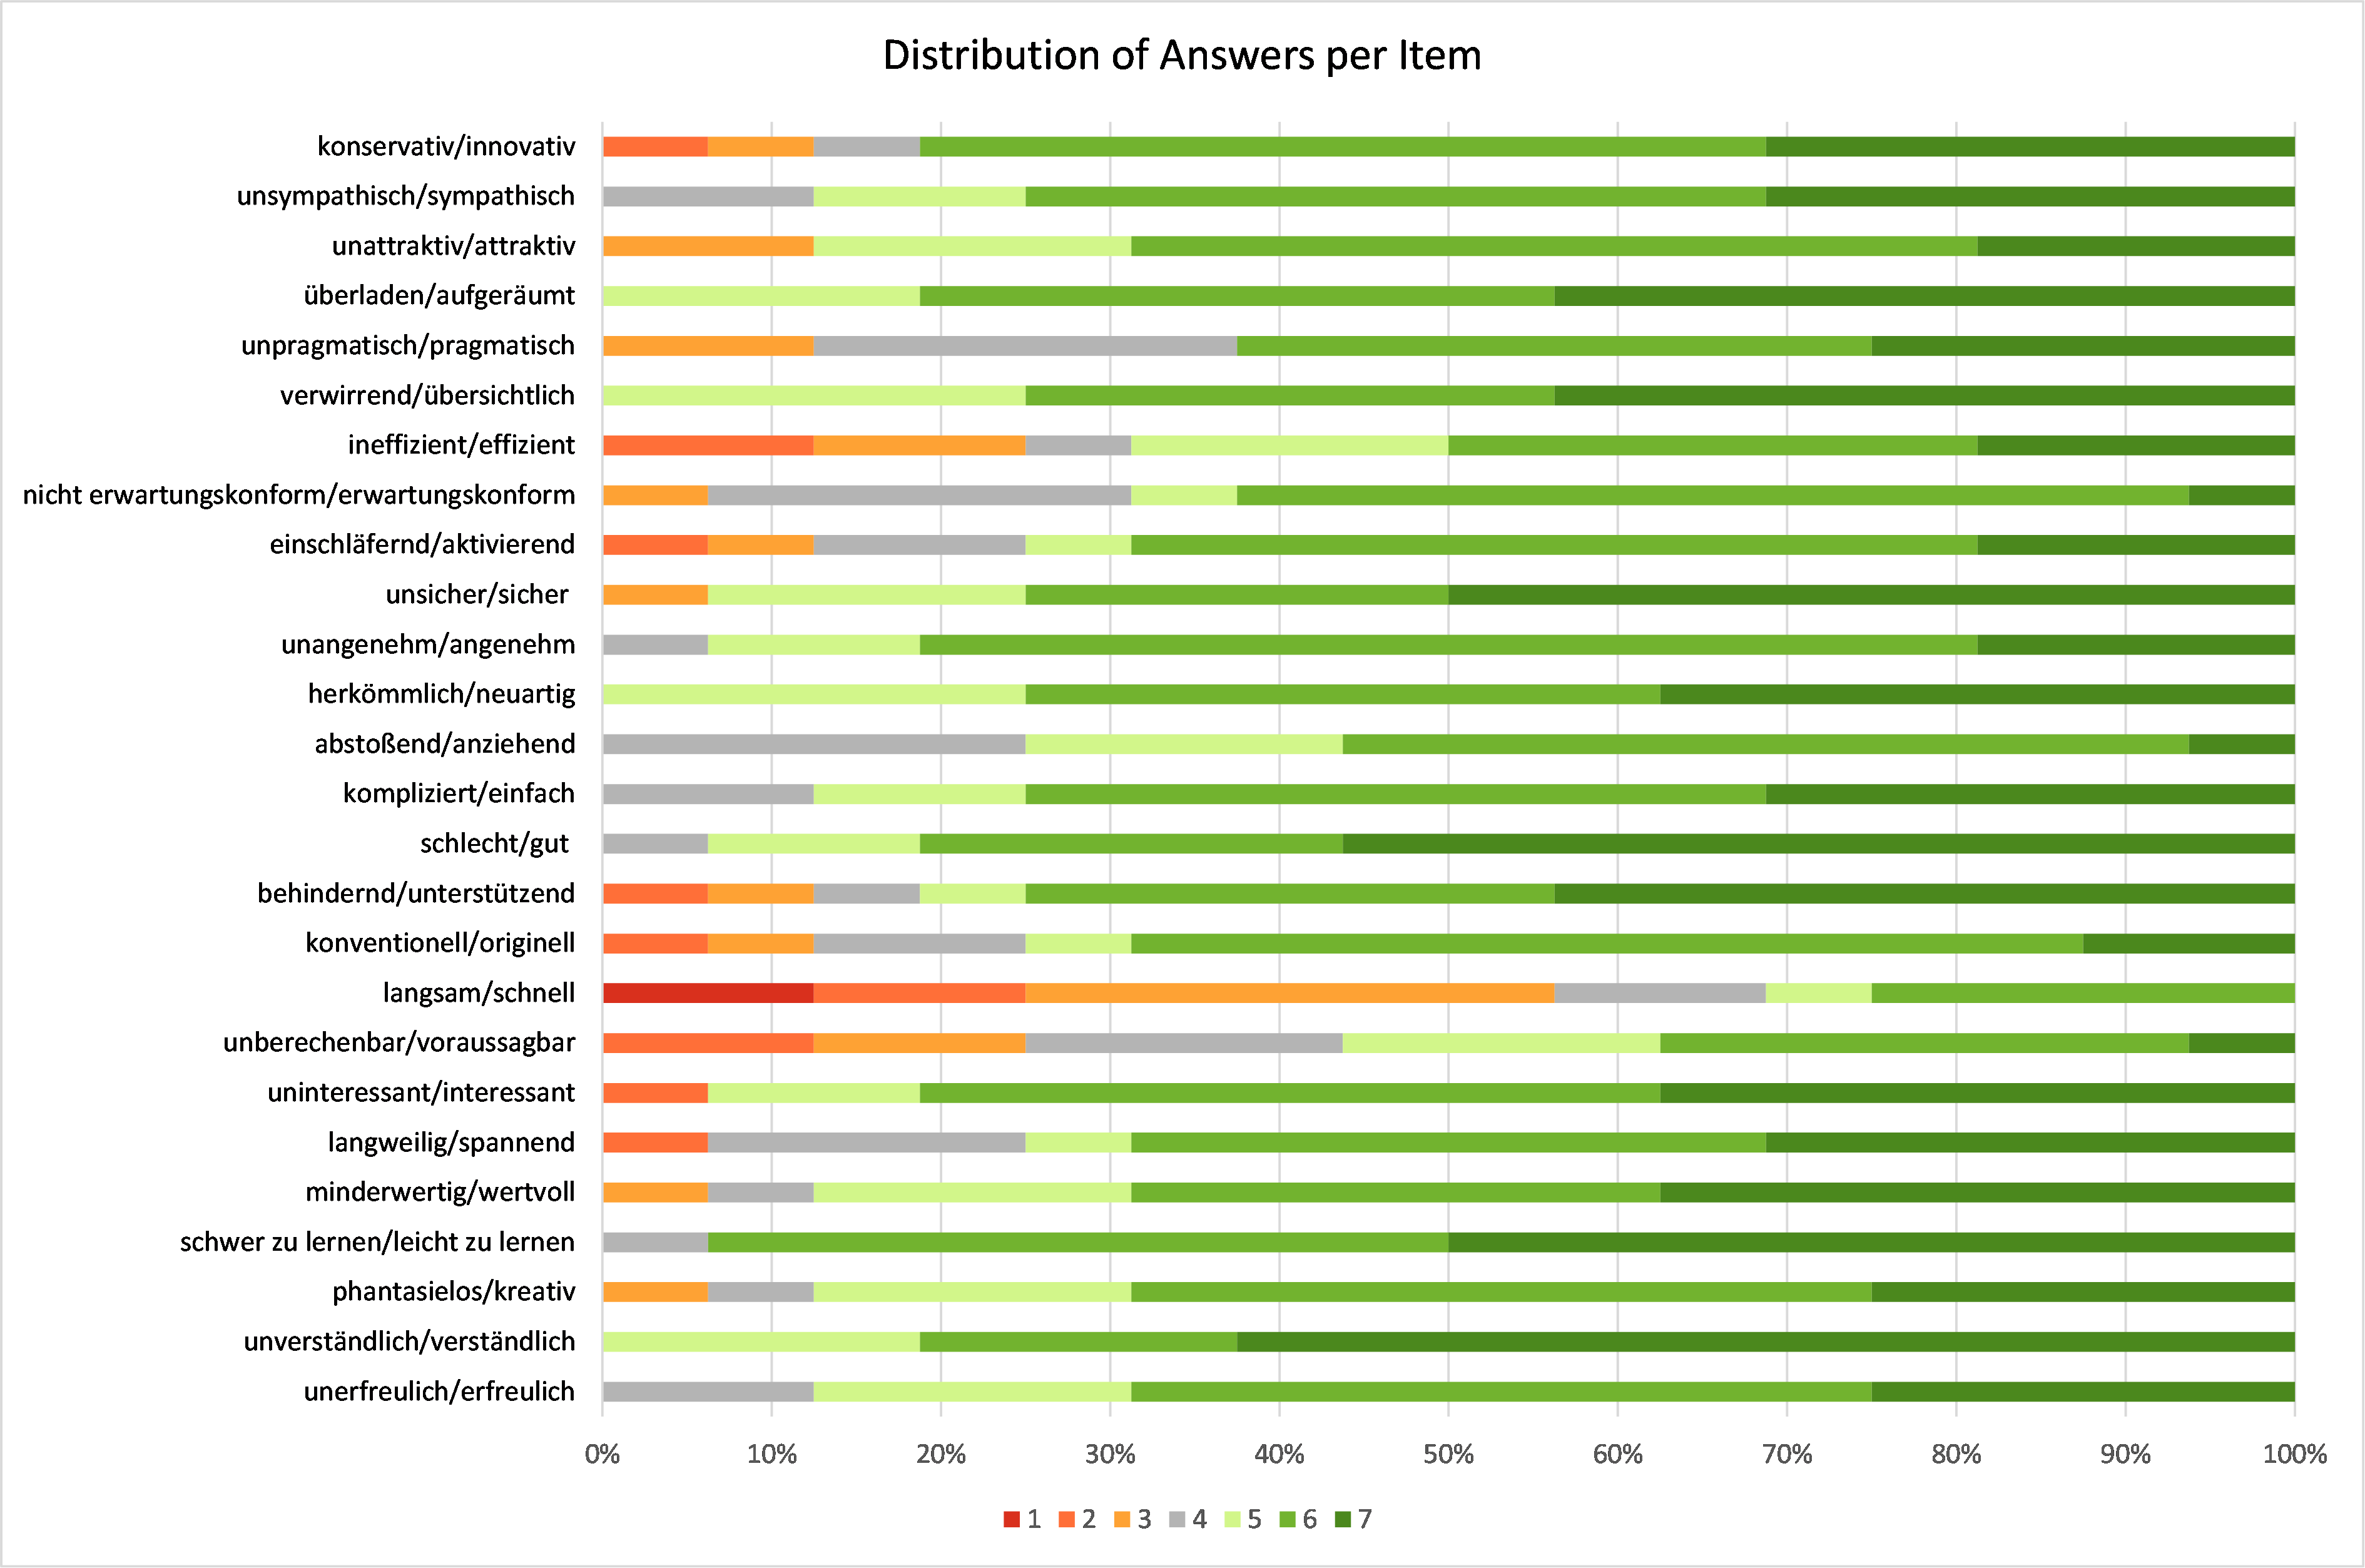
\includegraphics[scale=0.75]{images/Results/UEQ-VerteilungDerItems-CartesianScanning.png}
    \caption{Genaue Verteilung der Bewertungen der Items des UEQ beim Cartesian Scanning}
    \label{fig:ueqItemVerteilungCartesian}
\end{figure}

\cleardoublepage

\chapter{Projektdateien}

\section{Unity Projekt}
\label{Anhang:Projekt}

\cleardoublepage

